%%PREAMBLE %%%%%%%%%%%%%%%%%%%%%%%%%%%%
\documentclass[10pt, a4paper]{article}% size of txt = 10pt
\usepackage[top= 2cm,
			bottom = 2cm,
			left = 1.7cm,
			right = 1.7cm,
			footskip = 0.5cm,
			headsep = 0cm,
			headheight = 0cm
					]{geometry}
\usepackage{amsmath} % math packages
\usepackage{amsfonts}% math packages
\usepackage{amssymb} % math packages
\usepackage{graphicx} %package for including graphics
\usepackage{array}
\usepackage[thinlines]{easytable}
\usepackage{float}
\usepackage[section]{placeins}
\usepackage[hidelinks]{hyperref}
\usepackage[shortlabels]{enumitem}
\usepackage{svg}
\usepackage{bigstrut}
\usepackage{wrapfig,lipsum,booktabs}
\usepackage{subcaption}
\usepackage{xfrac}
\usepackage{pdfpages}
\usepackage{listings}
\usepackage{xcolor}

\usepackage{listings}
\usepackage{color} %red, green, blue, yellow, cyan, magenta, black, white
\definecolor{mygreen}{RGB}{28,172,0} % color values Red, Green, Blue
\definecolor{mylilas}{RGB}{170,55,241}

\definecolor{codegreen}{rgb}{0,0.6,0}
\definecolor{codegray}{rgb}{0.5,0.5,0.5}
\definecolor{codepurple}{rgb}{0.58,0,0.82}
\definecolor{backcolour}{rgb}{1,1,1}

\lstdefinestyle{mystyle}{
    backgroundcolor=\color{backcolour},   
    commentstyle=\color{codegreen},
    keywordstyle=\color{magenta},
    numberstyle=\tiny\color{codegray},
    stringstyle=\color{codepurple},
    basicstyle=\ttfamily\footnotesize,
    breakatwhitespace=false,         
    breaklines=true,                 
    captionpos=b,                    
    keepspaces=true,                 
    numbers=left,                    
    numbersep=5pt,                  
    showspaces=false,                
    showstringspaces=false,
    showtabs=false,                  
    tabsize=2
}
\lstset{style=mystyle}


%date format
\def\mydate{\leavevmode\hbox{\twodigits\day.\twodigits\month.\the\year}}
\def\twodigits#1{\ifnum#1<10 0\fi\the#1}


\usepackage[T1]{fontenc} 
\usepackage{lmodern}
\usepackage{indentfirst}
\setlength{\parindent}{1cm}

\makeatletter
\newcommand{\thickhline}{%
    \noalign {\ifnum 0=`}\fi \hrule height 2pt
    \futurelet \reserved@a \@xhline
}
\newcolumntype{"}{@{\hskip\tabcolsep\vrule width 2pt\hskip\tabcolsep}}
\makeatother
\newcolumntype{?}{!{\vrule width 2pt}}
%%DOC ENVIROMENT%%%%%%%%%%%%%%%%%%%%%%%
\begin{document}
%Title 
\begin{flushleft}%% left justification
	\textbf{\Large{MKC-DVV: Laboratorní úloha č.2}}\hfill Filip Paul\\
	\large{Komprimace MPEG-2 a zabezpečení videosignálu FEC \hfill\mydate}

\end{flushleft}
\section{\Large Porovnání výsledků měření:}
Bohužel jsem si neuložil výsledky chybovosti BER pro všechna měření (jak je napsáno v návodu).
Samotný BER by asi bylo možno získat porovnáváním vstupního souboru .m2v s výstupním souborem .m2v.
Do tohoto kroku jsem se však nepouštěl a výsledné hodnocení je tak vztaženo k subjektivnímu
vjemu výsledné kvality obrazu po dekódování.

\noindent Porovnávané výstupy jsou vztaženy k modelu kanálu tvořeného dolní propustí FIR filtru s parametry:
\begin{itemize}
    \item Mezní kmitočet: 0.45
    \item Řád filtru: 31
    \item Váhovací posloupnost: Hammingovo okno
\end{itemize}
Parametry filtru byly voleny metodou "pokus omyl" tak, aby se pro každé kódování nacházely ve výsledném dekódovaném videu alespoň nějaké artefakty.
Následující obrázky jsou screenshoty z dekódovaných videí. Zcela jednoznačně lze říci, že nejhorší kvalitu má kódování DVB-C, kde je obraz
pro zvolený filtr už téměř nerozpoznatelný v celé délce videa. Toto kódování má však nejnižší redundanci a generovaný soubor ".fec" má poloviční
velikost oproti DVB-S a DVB-T.
Kódování DVB-T a DVB-S jsou z hlediska kvality obrazu velmi podobná. Zde mohou být mírně zavádějící screenshoty obou kódování, kde je pro DVB-S patrný
artefakt v obrazu zatímco DVB-T je zcela bez artefaktů. Nicméně to platí pouze pro daný okamžik videa.\\
DVB-T a DVB-S kódování však mají větší redundanci oproti DVB-C a s tím související vyšší náročnost na kódování/dekódování.


\begin{figure}[ht!]
    \centering
    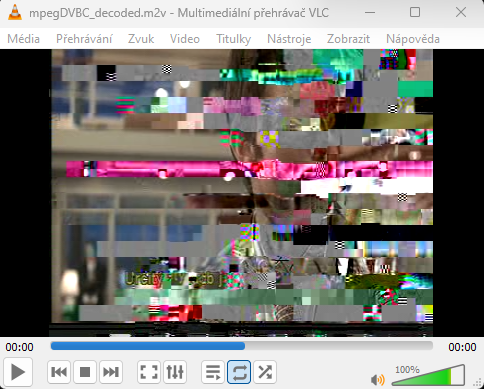
\includegraphics[width=0.7\textwidth]{DVBC.png}
    \caption{DVB-C}    
\end{figure}
\clearpage
\begin{figure}[ht!]
    \centering
    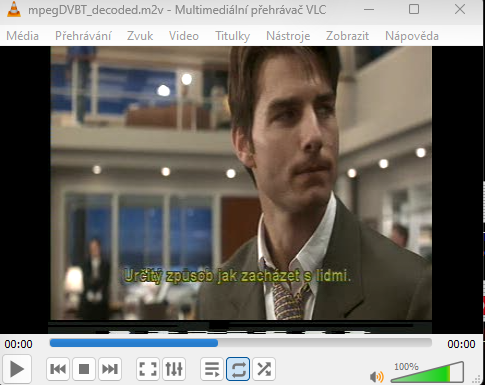
\includegraphics[width=0.7\textwidth]{DVBT.png}
    \caption{DVB-T}    
\end{figure}

\begin{figure}[ht!]
    \centering
    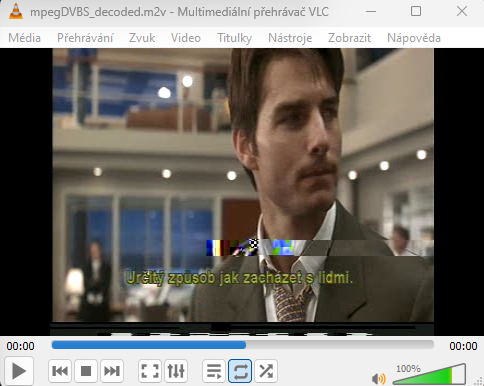
\includegraphics[width=0.7\textwidth]{DVBS.png}
    \caption{DVB-S}    
\end{figure}

Podpis je přiložen v protokolu z laboratorní úlohy č.6.

\end{document}

%\[f(x)= (x+2)^2 - \frac{9\cdot 2\pi}{26}\] %%mathematic equatation in display style mode
%%optional:
%	\begin{align} %%this alignes all charakters after & if *is removed equations will be numbered
%	\hspace{5cm}  
%		 x &= a_2 x^2 +_1 x + a_0 \\
% 		x &=x^2 \nonumber		%no number will not add number to eq
%	\end{align}


